\newpage
\section{Attività di analisi dei requisiti}
\subsection{Resoconto delle attività di verifica}

Dopo aver redatto tutti i documenti presenti nella Revisione dei Requisiti, il team ha svolto le attività di verifica su di essi e sui processi analizzati. I documenti sono stati sottoposti al processo di analisi statica definito nel documento \NdP{}.
Prima è stata utilizzata la tecnica del Walkthrough, segnalando gli errori incontrati tramite una lettura approfondita in un'apposita lista presa in carico dal \ver{} per attuare la correzione del documento. In seguito la stessa lista è stata utilizzata per la tecnica dell'Inspection, che è servita ad individuare la presenza di nuovi errori utilizzando il confronto della lista di quelli commessi in precedenza.
In seguito i documenti sono stati interamente verificati secondo le metriche descritte nell'Appendice~\nameref{AppB:metric} e sono stati riportati i risultati ottenuti.

\subsection{Verifica dei processi}
\subsubsection{Schedule Variance}
Nel seguente grafico vengono riportati i valori ottenuti calcolando la Schedule Variance sui tempi di stesura di ogni documento rispetto ai tempi prefissati nel \PdP{}:

\begin{figure}[h!]
	\centering
	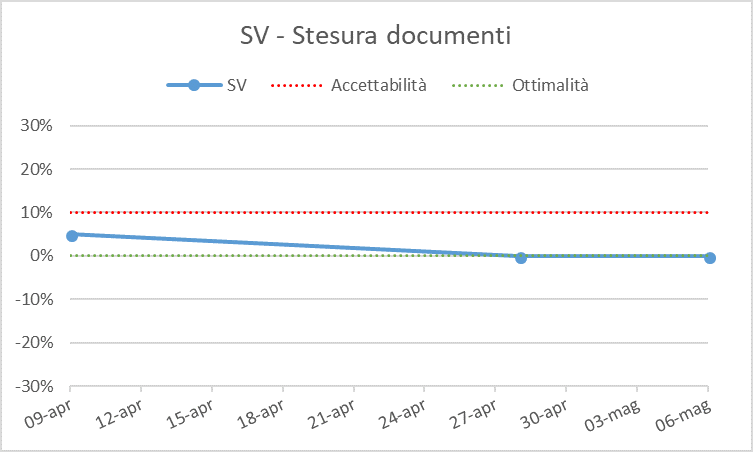
\includegraphics[scale=0.75]{img/Grafici/SV-Documenti.png}
		\caption{Schedule Variance per la stesura di ogni documento; \textcolor{green}{\checkmark} indica il raggiungimento della soglia di ottimalità, mentre \textcolor{red}{x} indica il non raggiungimento della soglia di accettabilità.}
	\label{fig:SV-Documenti}
\end{figure}

\begin{itemize}
	\item Schedule Variance finale: 0. 
	Il grafico evidenzia uno sforamento dei tempi riservati alla stesura delle \NdP{}, il quale viene però compensato da un anticipo sui tempi di stesura dello \SdF{}: il ritardo si quantifica in 2 giorni, esattamente come l'anticipo, mentre per la stesura degli altri documenti si sono rispettati i tempi previsti. 
	
	\item Soglia raggiunta: ottimalità.
\end{itemize}

\subsubsection{Cost Variance}
Il calcolo della Cost Variance sul processo di documentazione ha portato il seguente risultato: 

{
\renewcommand{\arraystretch}{2}
\centering
\begin{longtable}{| c | c | c | c | c |}
	\hline
	\textbf{Processo} & \textbf{BCWP} & \textbf{ACWP} & \textbf{CV} & \textbf{Valutazione} \\
	\hline
	Documentazione & 3870\euro & 3840\euro & 0,78\% & Ottimale \\
	\hline
	\caption{Calcolo della Cost Variance sul processo di documentazione}
\end{longtable}

}


\subsection{Verifica dei documenti}
\subsubsection{Schedule Variance}
Nel seguente grafico vengono riportati i valori ottenuti calcolando la Schedule Variance sui tempi di verifica di ogni documento rispetto ai tempi prefissati nel \PdP{}:

\begin{figure}[h!]
	\centering
	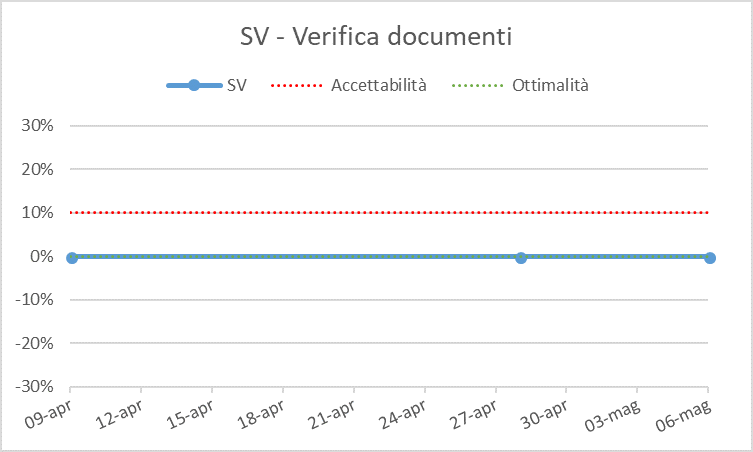
\includegraphics[scale=0.75]{img/Grafici/SV-VerDocumenti.png}
	\caption{Schedule Variance per la verifica di ogni documento; \textcolor{green}{\checkmark} indica il raggiungimento della soglia di ottimalità, mentre \textcolor{red}{x} indica il non raggiungimento della soglia di accettabilità.}
	\label{fig:SV-VerDocumenti}
\end{figure}

\begin{itemize}
	\item Schedule Variance finale: 0. 
	Il processo di verifica è stato completato senza anticipi né ritardi;
	
	\item Soglia raggiunta: ottimalità.
\end{itemize}


\subsubsection{Cost Variance}
Il calcolo della Cost Variance sul processo di verifica ha portato il seguente risultato: 

{
	\renewcommand{\arraystretch}{2}
	\centering
	\begin{longtable}{| c | c | c | c | c |}
		\hline
		\textbf{Processo} & \textbf{BCWP} & \textbf{ACWP} & \textbf{CV} & \textbf{Valutazione} \\
		\hline
		Verifica & 300\euro & 300\euro & 0\% & Ottimale \\
		\hline
		\caption{Calcolo della Cost Variance sul processo di verifica}
	\end{longtable}
	
}

\newpage

\subsubsection{Errori ortografici}
Durante l'ultima verifica, sono stati rilevati all'interno dei vari documenti alcuni errori ortografici, il cui numero è specificato nel seguente grafico:

\begin{figure}[h!]
	\centering
	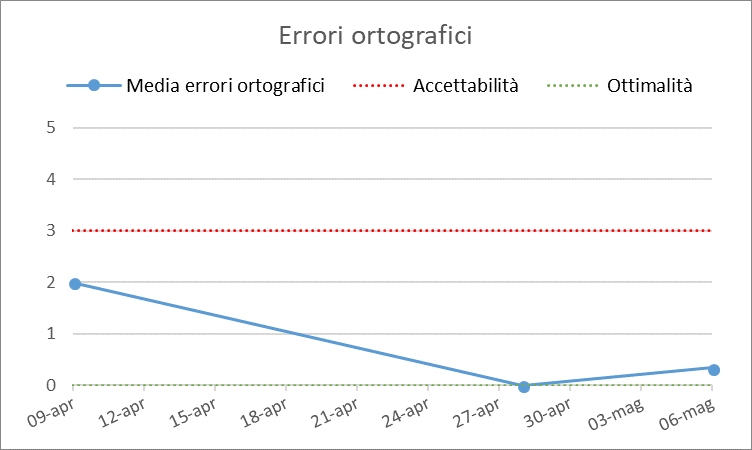
\includegraphics[scale=0.6]{img/Grafici/Errori_orto.png}
	\caption{Errori ortografici trovati in ogni documento; più il numero di errori è elevato, più ci si allontana dall'ottimalità.}
	\label{fig:Errori_orto}
\end{figure}

\begin{itemize}
\item Errori ortografici totali: 9.
\item Soglia raggiunta: con una media di 2 errori per documento, in generale si è rimasti dentro la soglia di accettabilità.
\end{itemize}

\subsubsection{Errori concettuali}

\begin{figure}[h!]
	\centering
	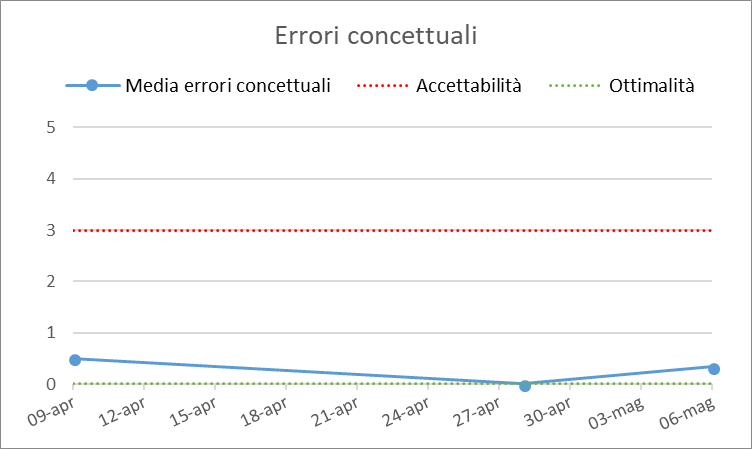
\includegraphics[scale=0.6]{img/Grafici/Errori_conce.png}
	\caption{Errori di concetto trovati in ogni documento; più il numero di errori è elevato, più ci si allontana dall'ottimalità.}
	\label{fig:Errori_conce}
\end{figure}

\begin{itemize}
	\item Errori concettuali totali: 3.
	\item Soglia raggiunta: con una media di 0,5 errori per documento, in generale si è rimasti ben dentro la soglia di accettabilità; in effetti la maggior parte dei documenti sono rimasti entro la soglia di ottimalità.
\end{itemize}

\subsubsection{Errori di forma}

\begin{figure}[h!]
	\centering
	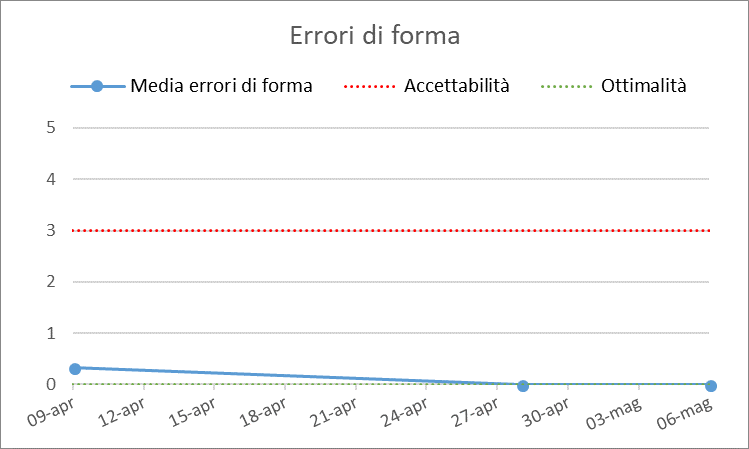
\includegraphics[scale=0.6]{img/Grafici/Errori_forma.png}
	\caption{Errori di forma trovati in ogni documento; più il numero di errori è elevato, più ci si allontana dall'ottimalità.}
	\label{fig:Errori_forma}
\end{figure}

\begin{itemize}
	\item Errori di forma totali: 3.
	\item Soglia raggiunta: con una media di 0,33 errori per documento, in generale si è rimasti ben dentro la soglia di accettabilità; in effetti la maggior parte dei documenti sono rimasti entro la soglia di ottimalità.
\end{itemize}

\newpage

\subsubsection{Indice Gulpease}

Tutti i documenti consegnati sono stati sottoposti al calcolo dell'Indice Gulpease per valutarne il grado di leggibilità, il quale è riportato nel seguente grafico:

\begin{figure}[h!]
	\centering
	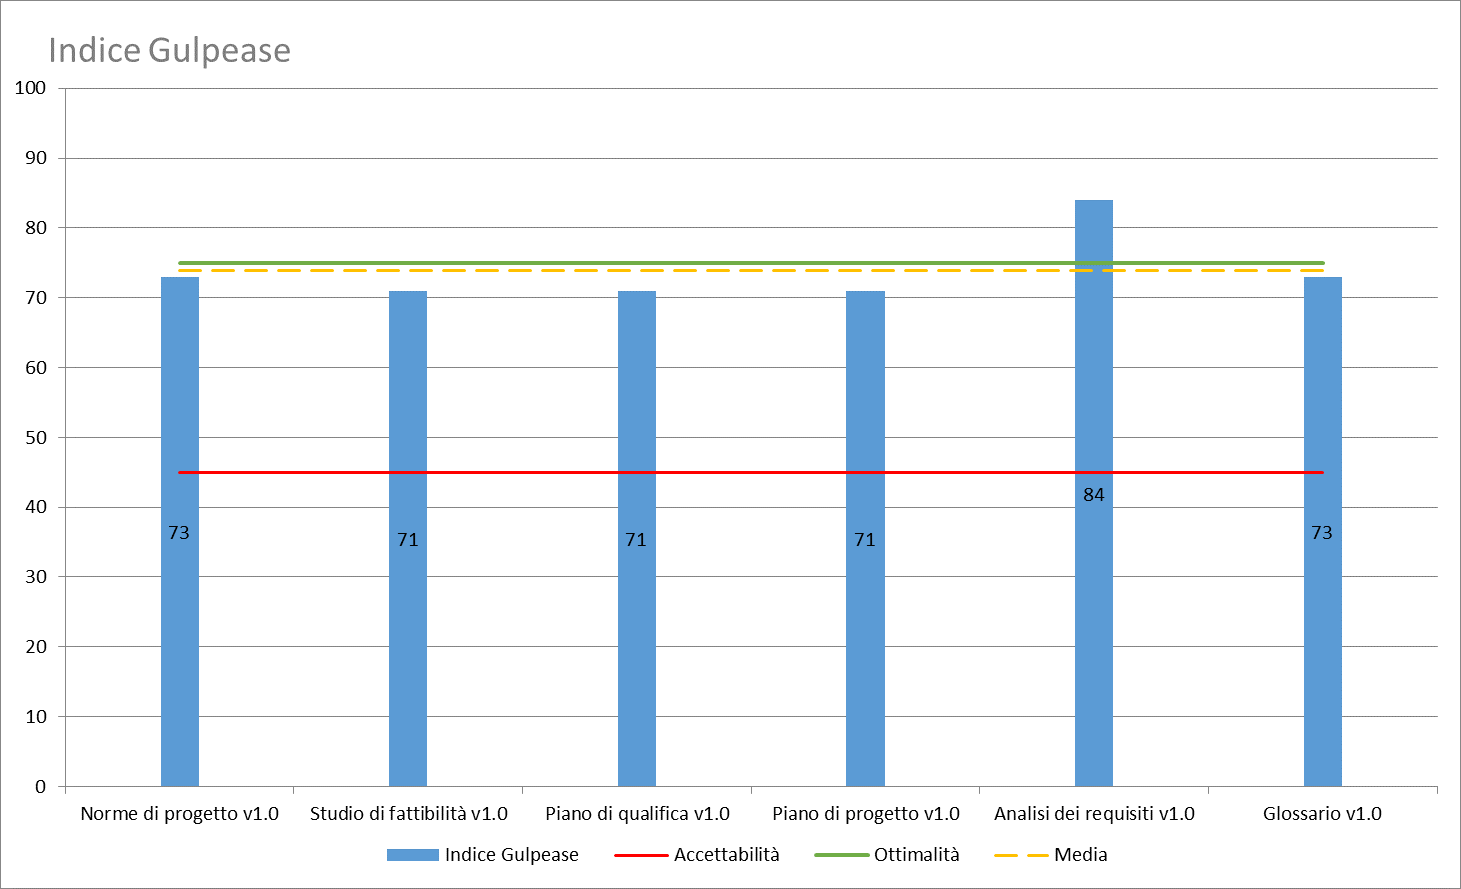
\includegraphics[scale=0.6]{img/Grafici/Gulpease.png}
	\caption{Indice Gulpease di ogni documento; più il valore è alto, più ci si avvicina all'ottimalità.}
	\label{fig:Gulpease}
\end{figure}

\begin{itemize}
	\item Soglia raggiunta: con una media di 73,84 punti, in generale si è rimasti dentro la soglia di accettabilità, arrivando poco sotto all'ottimalità.
\end{itemize}

